% Adjust these for the path of the theme and its graphics, relative to this file
%\usepackage{beamerthemeFalmouthGamesAcademy}
\usepackage{../../beamerthemeFalmouthGamesAcademy}
\usepackage{multimedia}
\graphicspath{ {../../} }

% Default language for code listings
\lstset{language=C++,
        morekeywords={each,in,nullptr}
}

% For strikethrough effect
\usepackage[normalem]{ulem}
\usepackage{wasysym}

\usepackage{pdfpages}

% http://www.texample.net/tikz/examples/state-machine/
\usetikzlibrary{arrows,automata}

\newcommand{\modulecode}{COMP260}\newcommand{\moduletitle}{Distributed Systems}\newcommand{\sessionnumber}{5}

\begin{document}
\title{\sessionnumber: Computing Foundations}
\subtitle{\modulecode: \moduletitle}

\frame{\titlepage} 

\begin{frame}{Learning outcomes}
	By the end of today's session, you will be able to:
	\begin{itemize}
		\item \textbf{Recall} the historical context of computing and gaming technology
		\item \textbf{Explain} the basic architecture of a computer
		\item \textbf{Distinguish} the most common programming languages and paradigms in use today
	\end{itemize}
\end{frame}

\begin{frame}{Today's agenda}
	\begin{itemize}
		\item COMP110 course outline
		\item History of computing
		\item Computer architecture
		\item Programming languages and paradigms
	\end{itemize}
\end{frame}

\part{Course introduction}
\frame{\partpage}

\begin{frame}{From the module guide}
This module will introduce you to the techniques of 3D graphics rendering and physics simulation used in modern computer games. Using the OpenGL library, you will develop an understanding of the 3D graphics pipeline, and how to program the GPU to produce advanced graphical effects.
\end{frame}

\begin{frame}{Topic schedule}
	\begin{center}
		On LearningSpace...
	\end{center}
\end{frame}

\begin{frame}{Assignment 1: Portfolio task}
	\begin{center}
		First worksheet is due in week 4.
	\end{center}
\end{frame}

\begin{frame}{Assignment 2: Research journal}
	\begin{center}
		First component due in week 3.
		\pause Don't forget to update the wiki!
	\end{center}
\end{frame}


\newcommand{\pictureslideb}[3]{
	\begin{frame}{#1}
		\begin{center}
			#3
			
			\vspace{6pt}
			
			\includegraphics[height=0.6\textheight]{#2}
		\end{center}
	\end{frame}
}

\newcommand{\pictureslide}[2]{
	\begin{frame}{#1}
		\begin{center}
			\includegraphics[height=0.6\textheight]{#2}
		\end{center}
	\end{frame}
}

\part{What was the first computer?}
\frame{\partpage}

\pictureslideb{Antikythera Mechanism ($\sim$150 BC)}{antikythera}{First mechanical computer?}
\pictureslideb{Babbage's Difference and Analytical Engines (1837)}{difference_engine}{First mechanical computer in modern age}
\pictureslideb{Colossus (1943)}{colossus}{First programmable electronic computer}
\pictureslideb{ENIAC (1946)}{eniac}{First general-purpose computer}
\pictureslideb{Manchester Small-Scale Experimental Machine (1948)}{manchester}{First stored program computer}
\pictureslideb{EDSAC (1949)}{edsac}{Many firsts in mathematics and science}
\pictureslideb{PDP-1 (1959)}{pdp1}{Influenced ``hacker culture''}
\pictureslideb{Datapoint 2200 (1970)}{datapoint2200}{First microcomputer}
\pictureslideb{Commodore VIC 20 (1980)}{vic20}{First computer to sell 1 million units}
\pictureslideb{IBM Personal Computer Model 5150 (1981)}{ibm_5150}{Precursor to the modern PC}

\part{What was the first computer game?}
\frame{\partpage}

\pictureslideb{Cathode Ray Tube Amusement Device (1948)}{crt}{First interactive electronic game}
\pictureslideb{Chess AI on the Ferranti Mark I (1951)}{ferranti}{First chess program}
\pictureslideb{Bertie the Brain (1950)}{bertie}{First computer game with a visual display}
\pictureslideb{OXO (1951)}{oxo}{First game with visuals on a general-purpose computer}
\pictureslideb{Tennis for Two (1959)}{tennis}{First to be created purely for entertainment}
\pictureslideb{SpaceWar! (1962)}{spacewar}{First widely available game, inspired first arcade games}
\pictureslideb{Pong (1972)}{pong}{First commercially successful game}

\part{What was the first games console?}
\frame{\partpage}

\pictureslideb{The Brown Box (1967)}{brownbox}{First prototype console}
\pictureslideb{Magnavox Odyssey (1972)}{magnavox}{First commercial console}

\begin{frame}{Game console timeline}
	\begin{center}
		\url{http://www.onlineeducation.net/videogame_timeline/video-game-timeline.jpg}
		
		(A little out of date!)
	\end{center}
\end{frame}


\part{Basic computer architecture}
\frame{\partpage}

\begin{frame}{What is a computer?}
	\begin{itemize}
		\item In \textbf{groups of 2-3}
		\item Discuss for \textbf{10 minutes}
		\item Go to \url{www.socrative.com} (or open the Socrative app) and enter room code \texttt{FALCOMPED}
		\item \textbf{Individually}, suggest a \textbf{one sentence} definition for a computer
	\end{itemize}
\end{frame}

\begin{frame}{The Von Neumann model}
	\begin{center}
		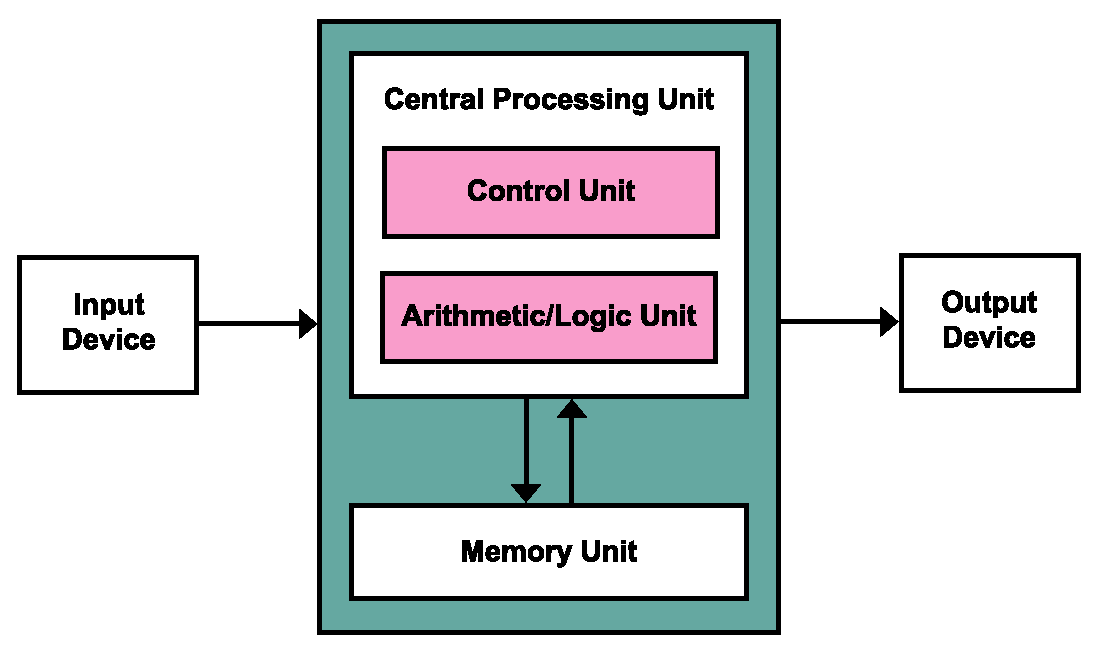
\includegraphics[height=0.7\textheight]{vonneumann}
	\end{center}
\end{frame}

\begin{frame}{Modern PC architecture}
	\begin{center}
		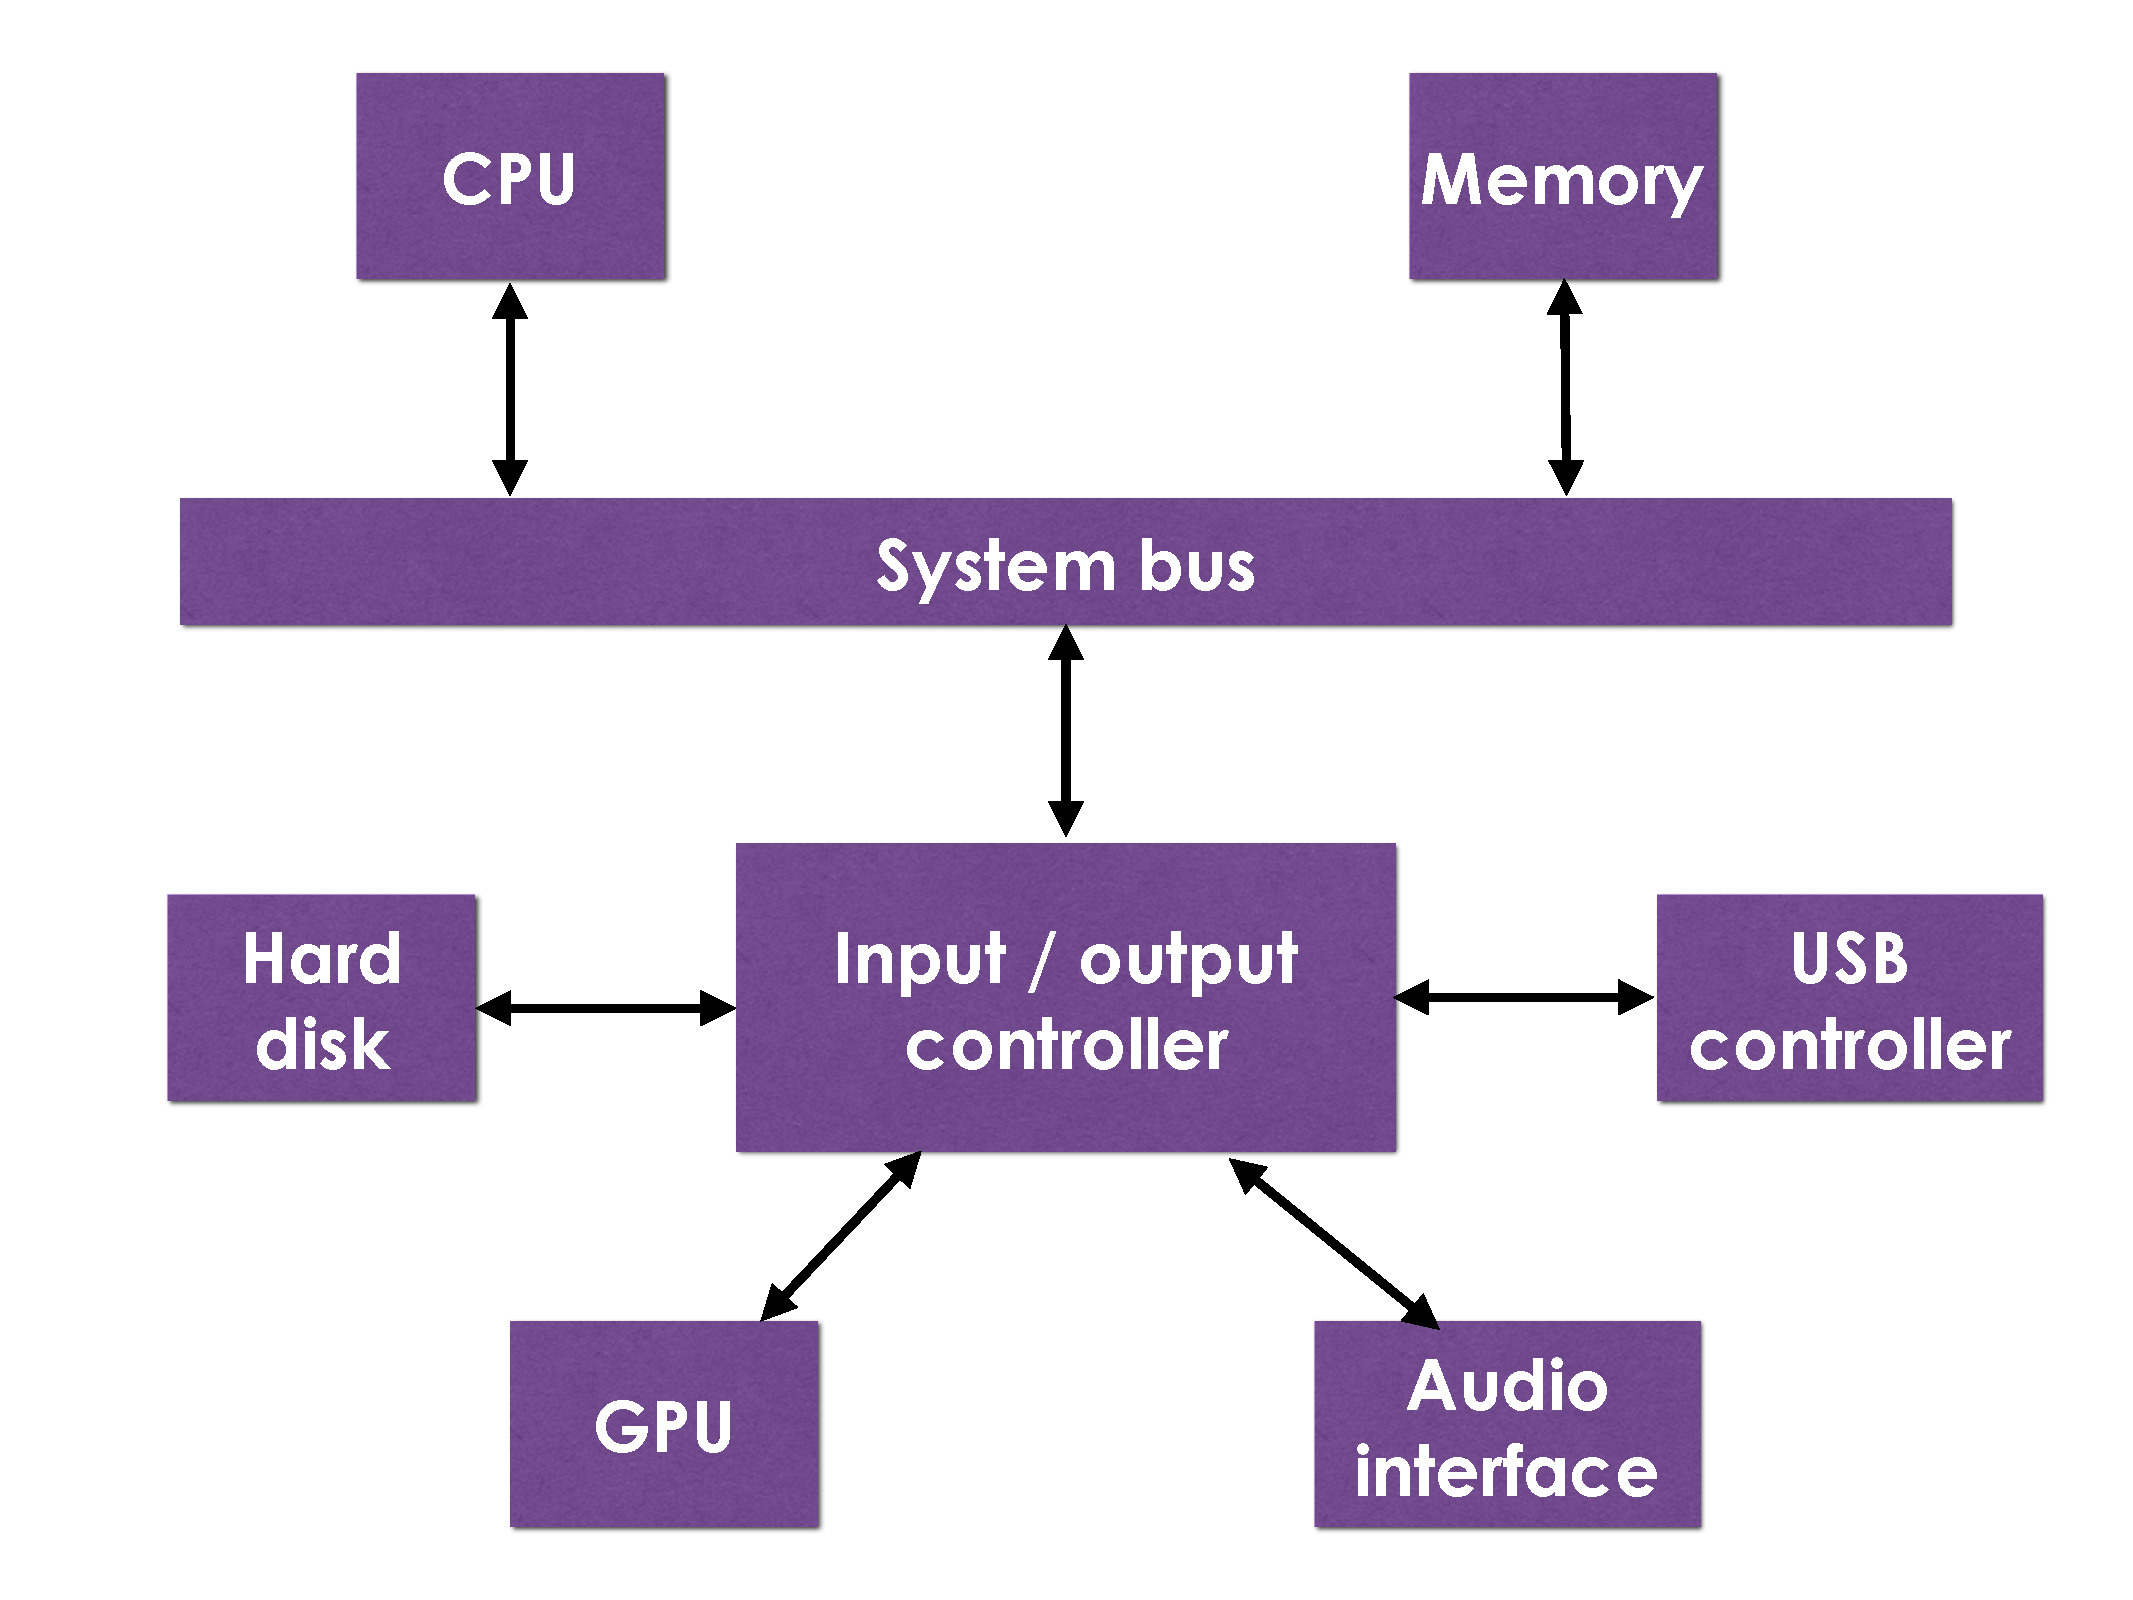
\includegraphics[height=0.7\textheight]{architecture-diagram}
	\end{center}
\end{frame}

\begin{frame}{Central processing unit (CPU)}
	\pause Carries out
	\begin{itemize}
		\pause \item Arithmetic operations
		\pause \item Logic operations
		\pause \item Control operations
	\end{itemize}
\end{frame}

\begin{frame}{Storage}
	\begin{itemize}
		\pause \item Primary storage
			\begin{itemize}
				\pause \item Directly accessible by the CPU
				\pause \item Random access memory (RAM)
				\pause \item Volatile --- loses its contents when switched off
			\end{itemize}
		\pause \item Secondary storage
			\begin{itemize}
				\pause \item E.g.\ hard disk, SSD, USB flash drive, DVD
				\pause \item Non-volatile --- keeps its contents when switched off
			\end{itemize}
	\end{itemize}
\end{frame}

\begin{frame}{Graphics processing unit (GPU)}
	\begin{itemize}
		\pause \item Responsible for displaying images on screen
		\pause \item Traditionally, one of many input/output devices
		\pause \item Nowadays, essentially a highly specialised CPU with its own primary storage
	\end{itemize}
\end{frame}

\begin{frame}{The stored program architecture}
	\begin{itemize}
		\pause \item A \textbf{computer program} is a sequence of instructions for the CPU
			\begin{itemize}
				\pause \item (Note: it's spelled ``program'', not ``programme'')
			\end{itemize}
		\pause \item The \textbf{programmable computer} --- can carry out different tasks depending on what program it is given
		\pause \item Most modern computers use the \textbf{same} memory to store the program and the data it uses
	\end{itemize}
\end{frame}



\part{Programming languages and paradigms}
\frame{\partpage}

\begin{frame}{What is a programming language?}
	\begin{itemize}
		\pause\item A \textbf{program} is a sequence of instructions for a computer to perform a specific task
		\pause\item A \textbf{programming language} is a formal language for communicating these sequences of instructions
	\end{itemize}
\end{frame}

\begin{frame}{Which is the best programming language?}
	\begin{itemize}
		\pause\item There is no ``best'' programming language
		\pause\item There are hundreds of programming languages, each better suited to some tasks than others
		\pause\item Sometimes your choice is dictated by your choice of platform, framework, game engine etc.
		\pause\item To become a better programmer (and maximise your employability)
			you should learn several languages (but one at a time!)
	\end{itemize}
\end{frame}

\begin{frame}{Low vs high level}
	\begin{itemize}
		\pause\item \textbf{Low level languages} give the programmer direct control over
			the hardware
		\pause\item \textbf{High level languages} give the programmer \textbf{abstraction},
			hiding the details of the hardware
		\pause\item High level languages trade efficiency for ease of programming
		\pause\item Lower level languages were once the choice of game programmers,
			but advances in hardware mean that higher level languages are often a
			better choice
	\end{itemize}
\end{frame}

\begin{frame}{Programming paradigms}
	\begin{itemize}
		\pause\item \textbf{Imperative}: program is a simple sequence of instructions,
			with \textbf{goto} instructions for program flow
		\pause\item \textbf{Structured}: like imperative, but with \textbf{control structures}
			(loops, conditionals etc.)
		\pause\item \textbf{Procedural}: structured program is broken down into
			\textbf{procedures}
		\pause\item \textbf{Object-oriented}: related procedures and data are grouped into
			\textbf{objects}
		\pause\item \textbf{Functional}: procedures are treated as mathematical objects that
			can be passed around and manipulated
		\pause\item \textbf{Declarative}: does not define the control flow of a program,
			but rather defines logical relations
	\end{itemize}
\end{frame}

\begin{frame}{Which paradigm?}
	\begin{itemize}
		\pause\item \textbf{Imperative} and \textbf{structured} languages are mainly of
			historical interest
		\pause\item Most commonly used languages today are a mixture of \textbf{procedural}
			and \textbf{object-oriented} paradigms, with many also incorporating
			ideas from \textbf{functional} programming
		\pause\item Purely \textbf{functional} languages (e.g.\ Haskell, F\#) are mainly used in academia,
			but favoured by some programmers
		\pause\item Purely \textbf{declarative} languages have uses in academia and some special-purpose languages
	\end{itemize}
\end{frame}

\begin{frame}{Machine code}
	\begin{columns}
		\begin{column}{0.4\textwidth}
			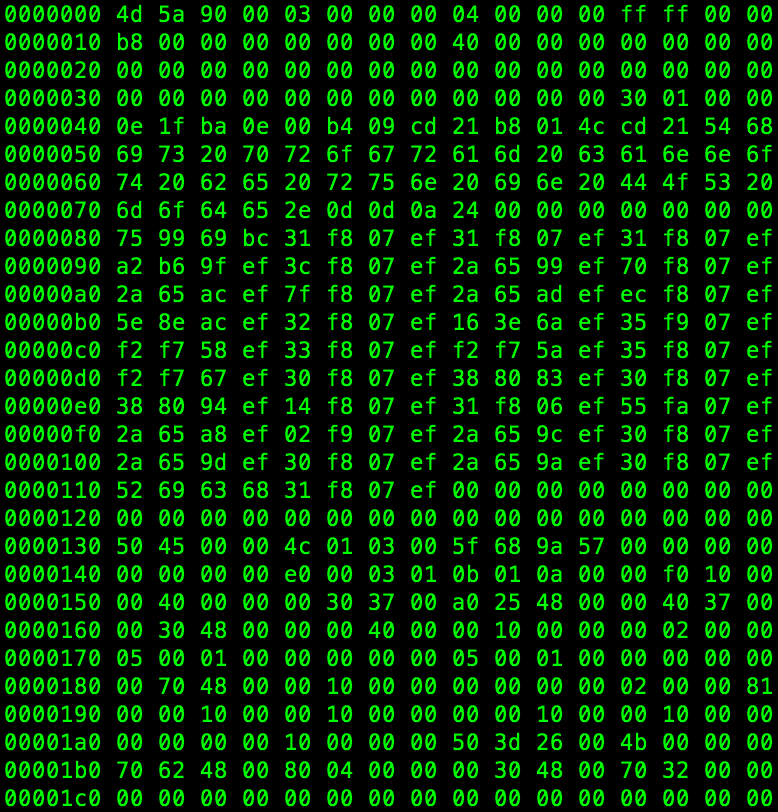
\includegraphics[width=\textwidth]{machinecode}
		\end{column}
		\begin{column}{0.58\textwidth}
			\begin{itemize}
				\pause\item Programs are represented as sequences of \textbf{numbers}
					specifying \textbf{machine instructions}
				\pause\item More on this later in the module
				\pause\item Nobody has actually written programs in machine code since the 1960s...
			\end{itemize}
		\end{column}
	\end{columns}
\end{frame}

\begin{frame}{Assembly language}
	\begin{columns}
		\begin{column}{0.4\textwidth}
			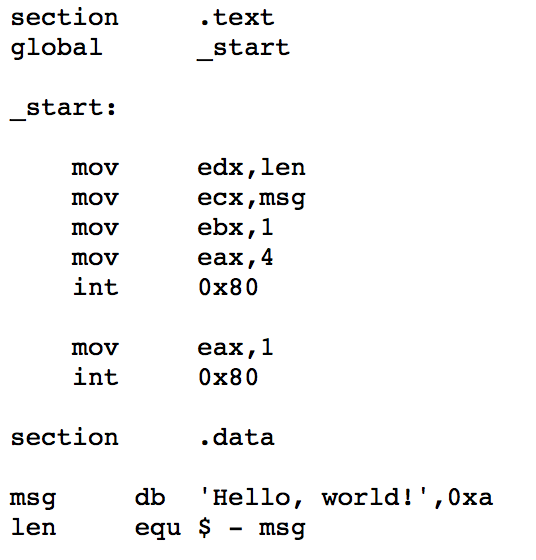
\includegraphics[width=\textwidth]{assembly}
		\end{column}
		\begin{column}{0.58\textwidth}
			\begin{itemize}
				\pause\item Each line of assembly code translates \textbf{directly} to an instruction of machine code
				\pause\item Commonly used for games in the 70s/80s/90s, but hardly ever used now
				\pause\item Allows very fine control over the hardware...
				\pause\item ... but difficult to use as there is no \textbf{abstraction}
				\pause\item Also not portable between CPU architectures
			\end{itemize}
		\end{column}
	\end{columns}
\end{frame}

\begin{frame}{C++}
	\begin{columns}
		\begin{column}{0.35\textwidth}
			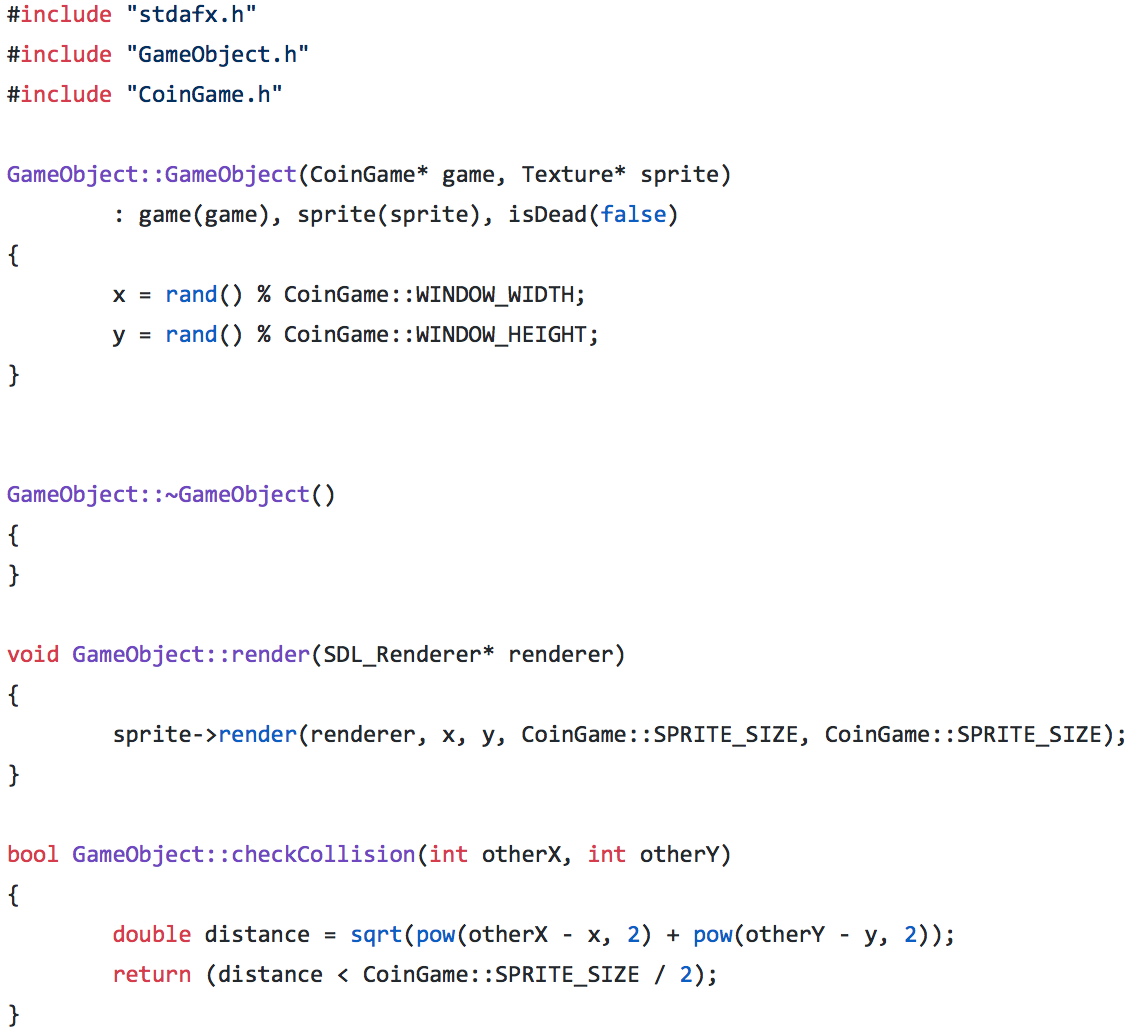
\includegraphics[width=\textwidth]{cplusplus}
		\end{column}
		\begin{column}{0.65\textwidth}
			\begin{itemize}
				\pause\item Initially an object-oriented extension for the procedural language C
				\pause\item Low level (though higher level than assembly)
				\pause\item Used by developers of game engines,
					and games using many popular ``AAA'' engines (Unreal, Source, CryEngine, ...)
				\pause\item Also used by developers of operating systems and embedded systems,
					but falling out of favour with other software developers
			\end{itemize}
		\end{column}
	\end{columns}
\end{frame}

\begin{frame}{High level languages in games}
	\pause Often favoured by smaller indie teams for rapid development
	\begin{itemize}
		\pause\item C\# (Unity)
		\pause\item Python (EVE Online, Pygame, Ren'py)
		\pause\item JavaScript/TypeScript (HTML5 browser games, Electron, node.js)
		\pause\item Objective-C, Swift (iOS games)
		\pause\item Java (Minecraft, Android games)
	\end{itemize}
	\pause There are many others, but these are the most commonly used in game development
\end{frame}

\begin{frame}{High level languages in other domains}
	\begin{itemize}
		\pause\item Data science: Python, R, Matlab, ...
		\pause\item Web: JavaScript, TypeScript, Python, Ruby, PHP, ...
		\pause\item Hardware: VHDL, MicroPython, ...
		\pause\item Creative computing: Processing, SuperCollider, Sonic Pi, ...
	\end{itemize}
\end{frame}

\begin{frame}{Scripting languages in games}
	\pause Many games use scripting languages in addition to their main development language
	\begin{itemize}
		\pause\item Lua (many AAA games)
		\pause\item Bespoke languages (many AAA games)
	\end{itemize}
	\pause Some game engines have their own scripting language
	\begin{itemize}
		\pause\item Blueprint (Unreal Engine)
		\pause\item GDScript (Godot)
		\pause\item GML (GameMaker)
	\end{itemize}
\end{frame}

\begin{frame}{Scripting languages}
	\pause Outside of games, ``scripting'' can refer to command-line scripting
	\begin{itemize}
		\pause\item Bash scripts (Unix)
		\pause\item Batch files, PowerShell (Windows)
	\end{itemize}
	\pause Some languages blur the line between scripting and programming, depending on usage
	\begin{itemize}
		\pause\item Python, Ruby, Perl, Lua...
	\end{itemize}
\end{frame}

\begin{frame}{Visual programming languages}
	\begin{columns}
		\begin{column}{0.4\textwidth}
			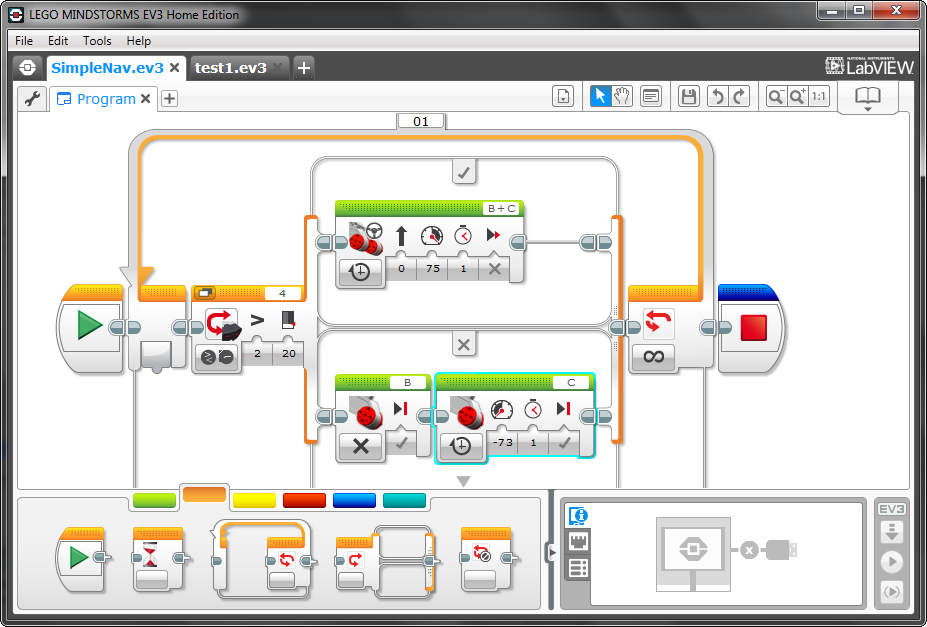
\includegraphics[width=\textwidth]{mindstorms}
			\par\vspace{2ex}\par
			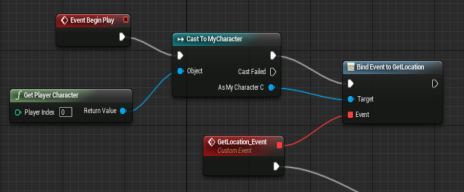
\includegraphics[width=\textwidth]{blueprint}
		\end{column}
		\begin{column}{0.58\textwidth}
			\pause Based on connecting graphical blocks rather than writing code as text
			\begin{itemize}
				\pause\item Scratch
				\pause\item Lego Mindstorms
				\pause\item Blueprint (Unreal)
			\end{itemize}
			\pause Note: despite the name, Microsoft Visual Studio is \textbf{not}
				a visual programming environment!
		\end{column}
	\end{columns}
\end{frame}

\begin{frame}{Special purpose languages}
	\begin{itemize}
		\pause\item SQL (database queries)
		\pause\item GLSL, HLSL (GPU shader programs)
		\pause\item LEX, YACC (script interpreters)
	\end{itemize}
\end{frame}

\begin{frame}{Markup languages}
	\pause Not to be confused with programming languages...
	\begin{itemize}
		\pause\item HTML, CSS (web pages)
		\pause\item LaTeX, Markdown (documentation)
		\pause\item XML, JSON (data storage)
	\end{itemize}
\end{frame}

\begin{frame}{Which programming language is most popular?}
	\begin{center}
		\url{http://githut.info}
	\end{center}
\end{frame}

\begin{frame}{``Family tree'' of programming languages}
	\begin{center}
		\url{https://www.levenez.com/lang/lang.pdf}
	\end{center}
\end{frame}


\begin{frame}{Debrief}
	\pause You should now be able to:
	\begin{itemize}
		\item \textbf{Recall} the historical context of computing and gaming technology
		\item \textbf{Explain} the basic architecture of a computer
		\item \textbf{Distinguish} the most common programming languages and paradigms in use today
	\end{itemize}
	\pause \textbf{Remember:} Worksheet A is due at \textbf{9am next Monday}!
\end{frame}

\end{document}
